\subsection{Parametrization of datapoints}
Additional to the reconstructed surface we need the following information for the least squares fit: 
\begin{itemize}
\item To which \ac{NURBS}-patch does each datapoint of the reconstructed surface belong to?
\item Which parameters $u,v$ does the datapoint have on this patch?
\end{itemize}
\subsubsection{Getting a coarse quad mesh \todourgent{better caption?}}
Before we can distribute datapoints to \ac{NURBS}-patches, we first have to find out how these patches look like. Since we want to have as few patches as possible we do not simply turn every \ac{quad} from the surface reconstruction into a patch. Instead of that we try to find a surface with as few \acp{quad} as possible, but still the same topology like our initially reconstructed surface. This coarse surface will be assumed to be the patch distribution for the later steps.

Therefore in our algorithm we are reconstructing the surface on two different scales, a coarse and a fine scale. The coarse scale surface reconstruction will be used as a patch distribution, from the fine scale we obtain our datapoints to which the \ac{NURBS} will be fitted to. We call this approach \emph{Twoscale \acl{DC}}(see \autoref{fig:TwoScale}).
Of course this simple approach comes with some drawbacks:
\begin{itemize}
\item We cannot guarantee that the coarse and the fine scale have the same topology. Topological details of the fine scale, which do not exist on the coarse scale, are lost.
\item Both resolutions have to be chosen manually, since we do not have a criterion for evaluating the quality of the coarse scale surface reconstruction.
\end{itemize}
\subsubsection{Projection of datapoints onto quads}
\todointern[inline]{go through formulation again}
Now that we have constructed a \ac{NURBS}-patch distribution we can estimate the parametrization of the datapoints on the fine scale by projecting the datapoints onto the patches: For this procedure we first have to find out onto which one of the patches one particular datapoint will be projected. Then we have to do the actual projection of the datapoint onto the quad: 
\begin{itemize}
\item The First can be done by simply measuring the distance from the datapoint to the centroid of each patch and deciding to project onto the patch with the smallest distance. 

\item For the latter we want the whole \ac{quad} to be parametrized on $u,v\in\left[0,1\right]^2$. We could either use bilinear interpolation for representing the quad and solve a non-linear minimization problem for each projection, or first approximate the quad with its least squares fit plane and then do a projection onto this plane by applying a simple basis transformation\footnote{This basis transformation can be computed in a very cheap way, by computing the QR-decomposition for the basis of each patch only once and applying it for each datapoint projected onto this patch.}. In our algorithm we used the second approach since the approximation of the original \acp{quad} via their least-squares fit planes introduces only a small error and significantly simplifies the projection onto the \ac{quad}.
\end{itemize}
\todourgent[inline]{more detail on this part? Perhaps in appendix?}
\todointern[inline]{making quads plane using least squares (Reference?), otherwise each projection is a non-linear optimization! show picture with both}
\todointern[inline]{coarse criterion: Distance to centroid (better: spacetree!)}
\todointern[inline]{fine criterion: Projection with QR decomposition}
Finally the projection of some datapoints might lead to parameters $u,v\not\in\left[0,1\right]^2$ in our algorithm we just omitted all those datapoints. If we do not get enough datapoints on each patch for the least squares fitting step after Peters' Scheme we artificially increase the number of datapoints by applying a subdivision scheme \todourgent{ref here?} to the fine scale surface reconstruction.

After having completed all these steps we obtain the following data for the subsequent steps of our algorithm:
\begin{itemize}
\item a coarse surface delivering the topology for our \ac{NURBS}-patches in Peters' Scheme
\item a set of datapoints from the fine scale with coordinates $\left(x,y,z\right)^T$ and parameters $\left(u,v\right)\in\left[0,1\right]^2$, where each datapoint is associated with a \ac{NURBS}-patch. 
\end{itemize}
For a visualization of our algorithm in 2D see \autoref{fig:TwoScale}.

\begin{figure}
\begin{center}
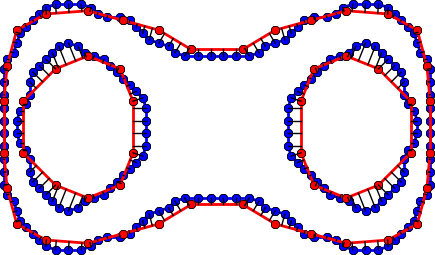
\includegraphics[width=.5 \textwidth]{Pictures/SurfaceReconstruction/TwoScale}
\caption{Twoscale \acl{DC} with a coarse surface reconstruction (red) and a fine one (blue). The datapoints from the fine scale are projected onto the edges from the coarse scale (black lines).}
\label{fig:TwoScale}
\end{center}
\end{figure}
\begin{comment}
\subsubsection{Parameter estimation}
\todo[inline]{explain different strategies, comparison of final results would be great (could also be part of third milestone?)}
\todo[inline]{show possible problems}
\end{comment}